% -*- mode: LaTeX; coding: utf-8 -*-
% Typeset with: XeLaTeX

\documentclass[a4paper,11pt]{article}
\usepackage{a4wide}

% Greek fonts
\RequirePackage{fontspec}
\defaultfontfeatures{Ligatures=TeX}
  % you may want to try: {Liberation Serif} or {Times New Roman}
\setmainfont{FreeSerif}
  % you may want to try: {Liberation Sans} or {Arial}
\setsansfont[Scale=MatchLowercase]{FreeSans}
  % you may want to try: {FreeMono} or {Courier New}
\setmonofont[Scale=MatchLowercase]{FreeMono}

\usepackage{amsmath}
\usepackage{hhline}
\usepackage{tikz}
\usetikzlibrary{positioning}


% Main document
\begin{document}
\title{Αλγοριθμική Επιστήμη Δεδομένων - 1η Σειρά Ασκήσεων}
\author{Θωμάς Παππάς}
\date{12 Μαΐου 2022}
\maketitle

\section*{Άσκηση 1}

\subsection*{Άσκηση 6.3.1 (MMDS)}

\paragraph{(a)} Το support για τα μεμονωμένα αντικείμενα, κάνοντας ένα πέρασμα από τα δεδομένα, είναι
\begin{center}
	% Result printed: [4, 6, 8, 8, 6, 4]
	\begin{tabular}{| r || c | c | c | c | c | c |}
		\hline
		item & $1$ & $2$ & $3$ & $4$ & $5$ & $6$ \\ \hline
		support & $4$ & $6$ & $8$ & $8$ & $6$ & $4$ \\ \hline
	\end{tabular}
\end{center}

ενώ για τα ζευγάρια αντικειμένων, χρησιμοποιώντας τη μέθοδο Multistage (με indexing structure Triangular-Matrix) βρίσκουμε ότι είναι
\begin{center}
	% Result printed: [2, 3, 2, 1, 0, 3, 4, 2, 1, 4, 4, 2, 3, 3, 2]
	\begin{tabular}{| c | c || c | c || c | c |}
		\hline
		pair & support & pair & support & pair & support \\ \hhline{|=|=#=|=#=|=|}
		$\{1,2\}$ & $2$ & $\{2,3\}$ & $3$ & $\{3,5\}$ & $4$ \\ \hline
		$\{1,3\}$ & $3$ & $\{2,4\}$ & $4$ & $\{3,6\}$ & $2$ \\ \hline
		$\{1,4\}$ & $2$ & $\{2,5\}$ & $2$ & $\{4,5\}$ & $3$ \\ \hline
		$\{1,5\}$ & $1$ & $\{2,6\}$ & $1$ & $\{4,6\}$ & $3$ \\ \hline
		$\{1,6\}$ & $0$ & $\{3,4\}$ & $4$ & $\{5,6\}$ & $2$ \\ \hline
	\end{tabular}
\end{center}

\paragraph{(b)} Χρησιμοποιώντας τον κανόνα $\{i,j\} \rightarrow i \times j \bmod 11$ βρίσκουμε ότι τα ζευγάρια αντικειμένων αντιστοιχίζονται στα hash buckets ως εξής:
\begin{center}
	\begin{tabular}{| c | c || c | c || c | c |}
		\hline
		pair & bucket & pair & bucket & pair & bucket \\ \hhline{|=|=#=|=#=|=|}
		$\{1,2\}$ & $2$ & $\{2,3\}$ & $6$ & $\{3,5\}$ & $4$ \\ \hline
		$\{1,3\}$ & $3$ & $\{2,4\}$ & $8$ & $\{3,6\}$ & $7$ \\ \hline
		$\{1,4\}$ & $4$ & $\{2,5\}$ & $10$ & $\{4,5\}$ & $9$ \\ \hline
		$\{1,5\}$ & $5$ & $\{2,6\}$ & $1$ & $\{4,6\}$ & $2$ \\ \hline
		$\{1,6\}$ & $6$ & $\{3,4\}$ & $1$ & $\{5,6\}$ & $8$ \\ \hline
	\end{tabular}
\end{center}

% Hash support on first pass: [0, 5, 5, 3, 6, 1, 3, 2, 6, 3, 2]
\paragraph{(c)} Από τα buckets που φτιάξαμε από το hash table στο 1ο πέρασμα, εφόσον αυξάνουμε κατά 1 το counter του κάθε bucket όταν συναντάμε ένα σύνολο που κάνει hash σε αυτό, παίρνουμε
\begin{center}
	\begin{tabular}{| r | c || r | c || r | c || r | c |}
		\hline
		bucket & count & bucket & count & bucket & count & bucket & count \\
		\hhline{|=|=#=|=#=|=#=|=|}
		$0$ & 0 & $3$ & 3 & $6$ & 3 & $9$ & 3 \\ \hline
		$1$ & 5 & $4$ & 6 & $7$ & 2 & $10$ & 2 \\ \hline
		$2$ & 5 & $5$ & 1 & $8$ & 6 &  & \\ \hline
	\end{tabular}
\end{center}
οπότε τα συχνά buckets είναι τα $1,2,4,8$.

\paragraph{(d)} Τα ζευγάρια που θα μετρηθούν στο 2ο πέρασμα του αλγόριθμου PCY είναι αυτά στα οποία και τα δύο στοιχεία είναι συχνά, αλλά και το ζευγάρι αντιστοιχεί σε hash bucket που είναι συχνός.
Εφόσον όλα τα μονοσύνολα είναι συχνά, από τα hash buckets παίρνουμε ότι θα μετρηθούν τα:
\begin{itemize}
	\item $\{2,6\},\{3,4\}$ (hash bucket $1$)
	\item $\{1,2\},\{4,6\}$ (hash bucket $2$)
	\item $\{1,4\},\{3,5\}$ (hash bucket $4$)
	\item $\{2,4\},\{5,6\}$ (hash bucket $8$)
\end{itemize}


\subsection*{Άσκηση 6.3.2 (MMDS)}
% Hash support on second pass: [0, 3, 2, 2, 0, 2, 4, 4, 5]
Τρέχουμε τον Multistage αλγόριθμο και κάνουμε hash τα στοιχεία που βρήκαμε συχνά στην Άσκηση 6.3.1 με το νέο hash κανόνα.
Το hash table που παίρνουμε είναι
\begin{center}
	\begin{tabular}{| r | c || r | c || r | c |}
		\hline
		bucket & count & bucket & count & bucket & count \\ \hhline{|=|=#=|=#=|=|}
		$0$ & 0 & $3$ & 2 & $6$ & 4 \\ \hline
		$1$ & 3 & $4$ & 0 & $7$ & 4 \\ \hline
		$2$ & 2 & $5$ & 2 & $8$ & 5 \\ \hline
	\end{tabular}
\end{center}
οπότε μόνο τα buckets $6,7,8$ γίνονται συχνά, και άρα τα υποψήφια ζευγάρια όντως μειώνονται στα
\[\{2,4\},\{2,6\},\{3,4\},\{3,5\}\]


\subsection*{Άσκηση 6.4.1}

Με οχτώ items $A,B,\dots,H$ και συχνά itemsets $\{A,B\},\{B,C\},\{A,C\},\{A,D\},\{E\},\{F\}$, το Negative Border αποτελείται από
\begin{itemize}
	\item τα μη συχνά 1-itemsets $\{G\},\{H\}$
	\item όλα τα μη συχνά 2-itemsets που είναι συνδυασμός από συχνά 1-itemsets, εδώ τα $A,B,\dots,F$
		\[
			\{A,E\},\{A,F\},\{B,D\},\{B,E\},\{B,F\},\{C,D\},\{C,E\},\{C,F\},\{D,E\},\{D,F\},\{E,F\}
		\]
	\item το $\{A,B,C\}$, το μοναδικό 3-itemset που έχει όλα τα υποσύνολά του συχνά
\end{itemize}

\section*{Άσκηση 2}

\paragraph{(α)} Η ορθότητα της μεθόδου A-priori βασίζεται στην αντι-μονοτονικότητα της συνάρτησης support, δηλαδή $\forall X,Y: X \subseteq Y$ έχουμε $\textnormal{support}(X) \geq \textnormal{support}(Y)$.
Από αυτό παίρνουμε ότι αν ένα itemset είναι συχνό, τότε και όλα τα υποσύνολά του είναι συχνά, και άρα στο βήμα παραγωγής υποψηφίων itemsets όπου βάζουμε μόνο αυτά που ικανοποιούν αυτή τη συνθήκη, ξέρουμε ότι δεν θα προσπεράσουμε κάποιο που είναι όντως συχνό.

Με αυτόν τον αλγόριθμο πραγματοποιούνται τόσες διασχίσεις στη βάση δεδομένων όσο και το μήκος του μεγαλύτερου συχνού itemset, αφού απαιτείται μετά από κάθε παραγωγή $C_i$ συνόλου.

\paragraph{(β)} Είναι πολυωνυμική ως προς την έξοδο, διότι όπως αναφέραμε και στο \textbf{(α)}, πραγματοποιούνται τόσες διασχίσεις στη βάση δεδομένων όσο και το μήκος του μεγαλύτερου συχνού itemset.

\paragraph{(γ)} Ο FP-Growth αρχικά χρειάζεται 2 περάσματα στη βάση δεδομένων ώστε να κατασκευάσει το FP-trie structure.
Από εκεί και πέρα θα χρειαστεί να διασχίσει το δέντρο σε κάθε βήμα ώστε να φτιάξει τα υποδέντρα, να κάνεις τις ανανεώσεις στις συχνότητες και να υπολογίσει το πλήθος των υπόλοιπων στοιχείων.
Εφόσον η διάσχιση του δέντρου μπορεί να γίνει σε γραμμικό χρόνο, η πολυπλοκότητα εξαρτάται πιο πολύ από τον αριθμό των βημάτων που θα χρειαστούν, δηλαδή πάλι ανάλογα με το μήκος του μεγαλύτερου συχνού itemset.
Οπότε και ο FP-Growth αλγόριθμος είναι πολυωνυμικός ως προς την έξοδο.
\\[8pt]
Για την πολυπλοκότητα του αλγορίθμου ίσως αξίζει να αναφέρουμε και τη σχέση που έχει ως προς το πλήθος των items $k$.
Tο μέγεθος του δέντρου που θα προκύψει εξαρτάται από το πόσες διαφορετικές λεξικογραφικές εγγραφές αποτελείται η βάση, όπου στη χειρότερη θα μπορούσε να είναι $2^k$.
Ο αλγόριθμος θα πρέπει να το διασχίσει τουλάχιστον $k$ φορές, μία για κάθε στοιχείο, οπότε στη χειρότερη έχουμε μια πολυπλοκότητα $\mathcal{O}(k2^k)$.
Εφόσον βέβαια το $k$ είναι μικρός αριθμός σε σχέση με το πλήθος των εγγραφών, ενώ επίσης έχουμε και τη γενική υπόθεση ότι τα συχνά υποσύνολα θα είναι πολύ λιγότερα από το μέγεθος της βάσης, μπορούμε να περιμένουμε ότι ακόμα και σε αυτήν την περίπτωση τα υποδέντρα που θα προκύψουν θα μικρύνουν μετά από ένα μικρό αριθμό βημάτων.

\paragraph{(δ)}
\subparagraph{Α-priori}
Ξεκινάμε με το 1ο πέρασμα της βάσης δεδομένων όπου μετράμε τα συχνά 1-itemsets $a,b,c,d$, τα οποία και βρίσκουμε ότι έχουν συχνότητα $7,6,7,9$ αντίστοιχα, οπότε
\[ L_1 = \{ \{a\},\{b\},\{c\},\{d\} \} \]
Οπότε όλα τα πιθανά 2-itemsets είναι candidate
\[ C_2 = \{ \{a,b\},\{a,c\},\{a,d\},\{b,c\},\{b,d\},\{c,d\} \} \]
τα οποία μετράμε στο 2ο πέρασμα της βάσης και βρίσκουμε ότι έχουν συχνότητα $2,4,5,3,5,4$ αντίστοιχα, οπότε με threshold $s=4$ παίρνουμε
\[ L_2 = \{ \{a,c\},\{a,d\},\{b,d\},\{c,d\} \} \]
Συνεχίζοντας για candidate 3-itemsets, αρχικά ψάχνουμε δύο συχνά 2-itemsets που διαφέρουν κατά ένα στοιχείο ώστε με την ένωσή τους να πάρουμε ένα 3-itemset, για το οποίο στη συνέχεια ελέγχουμε εάν όλα τα 2-itemset υποσύνολά του είναι επίσης συχνά.
Βρίσκουμε τα $\{a,c,d\},\{a,b,d\}$ από τους συνδυασμούς, αλλά το δεύτερο απορρίπτεται διότι το $\{a,b\}$ δεν είναι συχνό.
Οπότε
\[ C_3 = \{ \{a,c,d\} \} \]
το οποίο και μετράμε στη βάση (3ο πέρασμα) και βλέπουμε ότι δεν είναι συχνό.
Παίρνουμε λοιπόν $L_3 = \emptyset$ και σταματάμε.
\\[8pt]
Οπότε τα συχνά υποσύνολα της βάσης δεδομένων είναι τα
\[ \{ \{a,c\},\{a,d\},\{b,d\},\{c,d\} \} \]

\subparagraph{FP-Growth}
Ξεκινάμε όπως με τον A-priori και βρίσκουμε τα συχνά 1-itemsets $a,b,c,d$ με συχνότητα $7,6,7,9$ αντίστοιχα.
Κάνοντας ένα 2ο πέρασμα στη βάση ταξινομούμε τα στοιχεία σε κάθε itemset κατά φθίνουσα συχνότητα, δηλαδή $d,a,c,b$, και φτιάχνουμε το FP-trie.
\begin{center}
	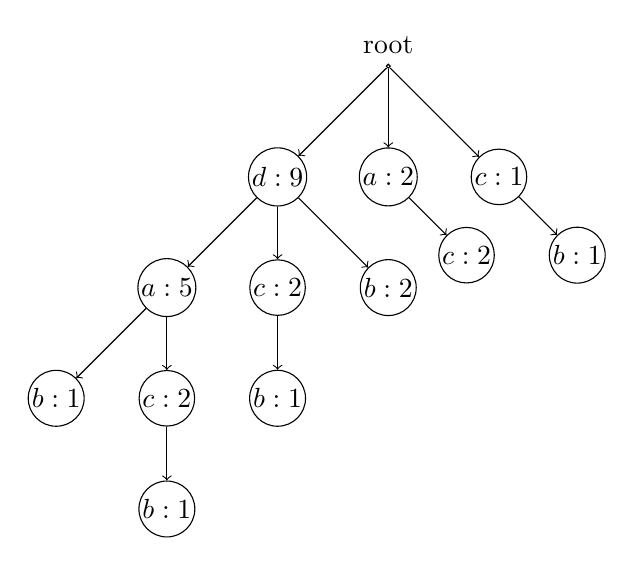
\begin{tikzpicture}[
			node distance=40pt,
			main/.style = {draw, circle, inner sep=.5pt}
		]
		\node[main, label=above:{root}] (r) {};
		% Level 1.
		\node[main, below of=r] (a) {$a:2$};
		\node[main, left of=a] (d) {$d:9$};
		\node[main, right of=a] (c) {$c:1$};
		% Level 2.
		\node[main, below of=d] (dc) {$c:2$};
		\node[main, left of=dc] (da) {$a:5$};
		\node[main, right of=dc] (db) {$b:2$};
		\node[main, below right of=a] (ac) {$c:2$};
		\node[main, below right of=c] (cb) {$b:1$};
		% Level 3.
		\node[main, below of=da] (dac) {$c:2$};
		\node[main, left of=dac] (dab) {$b:1$};
		\node[main, below of=dc] (dcb) {$b:1$};
		% Level 4.
		\node[main, below of=dac] (dacb) {$b:1$};

		\draw[->] (r) to (a);
		\draw[->] (r) to (d);
		\draw[->] (r) to (c);
		\draw[->] (d) to (dc);
		\draw[->] (d) to (da);
		\draw[->] (d) to (db);
		\draw[->] (a) to (ac);
		\draw[->] (c) to (cb);
		\draw[->] (da) to (dac);
		\draw[->] (da) to (dab);
		\draw[->] (dc) to (dcb);
		\draw[->] (dac) to (dacb);
	\end{tikzpicture}
\end{center}

Τώρα θα δούμε τα υποδέντρα που καταλήγουν σε κάθε στοιχείο.
Ξεκινάμε με το $b$ που έχει τη μικρότερη συχνότητα οπότε φτιάχνουμε το υποδέντρο μονοπατιών που καταλήγουν σε αυτό και ανανεώνουμε συχνότητες.
\begin{center}
	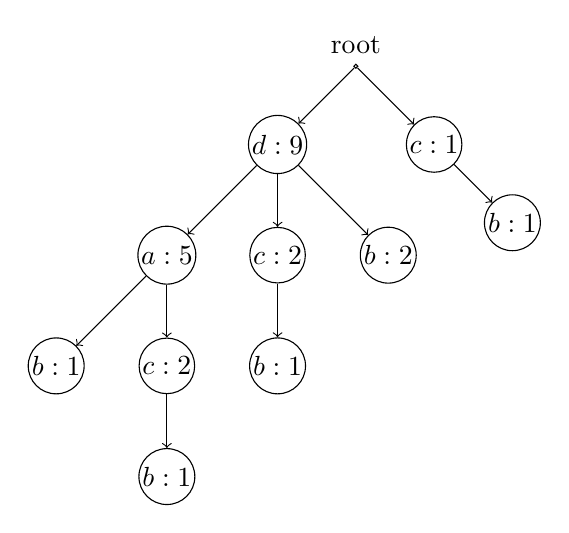
\begin{tikzpicture}[
			node distance=40pt,
			main/.style = {draw, circle, inner sep=.5pt}
		]
		\node[main, label=above:{root}] (r) {};
		% Level 1.
		\node[main, below left of=r] (d) {$d:9$};
		\node[main, below right of=r] (c) {$c:1$};
		% Level 2.
		\node[main, below of=d] (dc) {$c:2$};
		\node[main, left of=dc] (da) {$a:5$};
		\node[main, right of=dc] (db) {$b:2$};
		\node[main, below right of=c] (cb) {$b:1$};
		% Level 3.
		\node[main, below of=da] (dac) {$c:2$};
		\node[main, left of=dac] (dab) {$b:1$};
		\node[main, below of=dc] (dcb) {$b:1$};
		% Level 4.
		\node[main, below of=dac] (dacb) {$b:1$};
		
		\draw[->] (r) to (d);
		\draw[->] (r) to (c);
		\draw[->] (d) to (dc);
		\draw[->] (d) to (da);
		\draw[->] (d) to (db);
		\draw[->] (c) to (cb);
		\draw[->] (da) to (dac);
		\draw[->] (da) to (dab);
		\draw[->] (dc) to (dcb);
		\draw[->] (dac) to (dacb);
	\end{tikzpicture}
	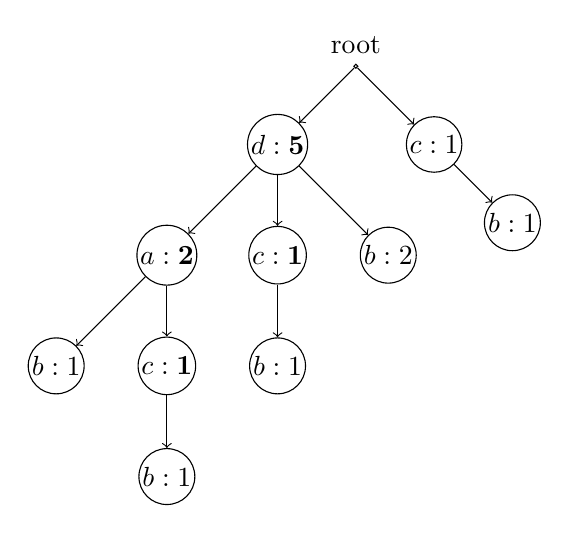
\begin{tikzpicture}[
			node distance=40pt,
			main/.style = {draw, circle, inner sep=.5pt}
		]
		\node[main, label=above:{root}] (r) {};
		% Level 1.
		\node[main, below left of=r] (d) {$d:\mathbf{5}$};
		\node[main, below right of=r] (c) {$c:1$};
		% Level 2.
		\node[main, below of=d] (dc) {$c:\mathbf{1}$};
		\node[main, left of=dc] (da) {$a:\mathbf{2}$};
		\node[main, right of=dc] (db) {$b:2$};
		\node[main, below right of=c] (cb) {$b:1$};
		% Level 3.
		\node[main, below of=da] (dac) {$c:\mathbf{1}$};
		\node[main, left of=dac] (dab) {$b:1$};
		\node[main, below of=dc] (dcb) {$b:1$};
		% Level 4.
		\node[main, below of=dac] (dacb) {$b:1$};
		
		\draw[->] (r) to (d);
		\draw[->] (r) to (c);
		\draw[->] (d) to (dc);
		\draw[->] (d) to (da);
		\draw[->] (d) to (db);
		\draw[->] (c) to (cb);
		\draw[->] (da) to (dac);
		\draw[->] (da) to (dab);
		\draw[->] (dc) to (dcb);
		\draw[->] (dac) to (dacb);
	\end{tikzpicture}
\end{center}
Μετράμε τις συχνότητες από τα υπόλοιπα στοιχεία ($a,c,d$) και βρίσκουμε $2,3,5$ αντίστοιχα οπότε εφόσον μόνο το $d$ βγαίνει πάνω από το threshold έχουμε ότι το $\{b,d\}$ συχνό.

Θα μπορούσαμε να συνεχίσουμε να ψάξουμε για συχνά 3-itemsets αλλά εφόσον δεν βρήκαμε άλλο συχνό 2-itemset που να περιέχει το $b$ τότε σίγουρα δεν υπάρχουν 3-itemsets που να το περιέχουν.
\\[8pt]
Ομοίως τώρα με το στοιχείο $c$.
\begin{center}
	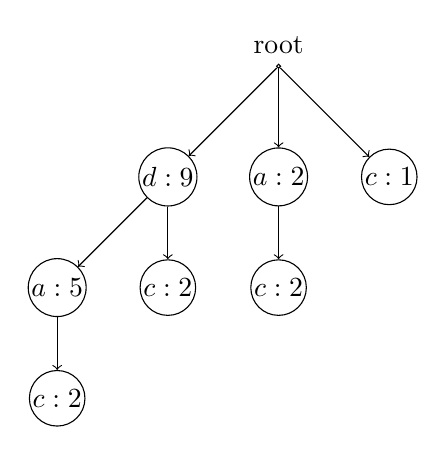
\begin{tikzpicture}[
			node distance=40pt,
			main/.style = {draw, circle, inner sep=.5pt}
		]
		\node[main, label=above:{root}] (r) {};
		% Level 1.
		\node[main, below of=r] (a) {$a:2$};
		\node[main, left of=a] (d) {$d:9$};
		\node[main, right of=a] (c) {$c:1$};
		% Level 2.
		\node[main, below of=d] (dc) {$c:2$};
		\node[main, left of=dc] (da) {$a:5$};
		\node[main, below of=a] (ac) {$c:2$};
		% Level 3.
		\node[main, below of=da] (dac) {$c:2$};
		
		\draw[->] (r) to (a);
		\draw[->] (r) to (d);
		\draw[->] (r) to (c);
		\draw[->] (d) to (dc);
		\draw[->] (d) to (da);
		\draw[->] (a) to (ac);
		\draw[->] (da) to (dac);
	\end{tikzpicture}
	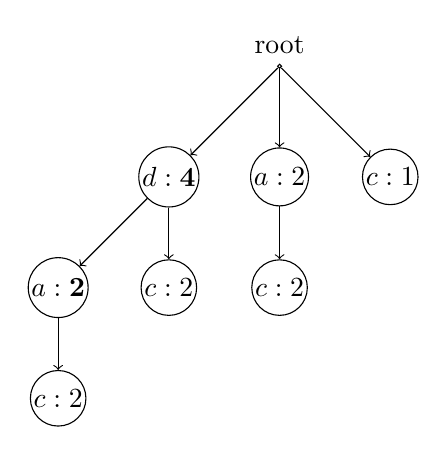
\begin{tikzpicture}[
			node distance=40pt,
			main/.style = {draw, circle, inner sep=.5pt}
		]
		\node[main, label=above:{root}] (r) {};
		% Level 1.
		\node[main, below of=r] (a) {$a:2$};
		\node[main, left of=a] (d) {$d:\mathbf{4}$};
		\node[main, right of=a] (c) {$c:1$};
		% Level 2.
		\node[main, below of=d] (dc) {$c:2$};
		\node[main, left of=dc] (da) {$a:\mathbf{2}$};
		\node[main, below of=a] (ac) {$c:2$};
		% Level 3.
		\node[main, below of=da] (dac) {$c:2$};
		
		\draw[->] (r) to (a);
		\draw[->] (r) to (d);
		\draw[->] (r) to (c);
		\draw[->] (d) to (dc);
		\draw[->] (d) to (da);
		\draw[->] (a) to (ac);
		\draw[->] (da) to (dac);
	\end{tikzpicture}
\end{center}
Βρίσκουμε συχνότητα για το $a$ ίση με $2+2=4$ και για το $d$ επίσης $4$.
Οπότε έχουμε συχνά 2-itemsets τα $\{a,c\},\{c,d\}$.

Συνεχίζουμε για 3-itemsets με μόνο υποψήφιο το $\{a,c,d\}$ οπότε χρησιμοποιώντας το $\{c,d\}$ παίρνουμε το υποδέντρο με τα μονοπάτια που το περιέχει, ανανεώνουμε συχνότητες (πάλι εδώ δεν χρειάζεται) και μετά μετράμε συχνότητα για το $a$.
(Tο ίδιο αποτέλεσμα θα πάρουμε και εάν χρησιμοποιήσουμε το $\{a,c\}$ και μετά μετρήσουμε τη συχνότητα του $d$)
\begin{center}
	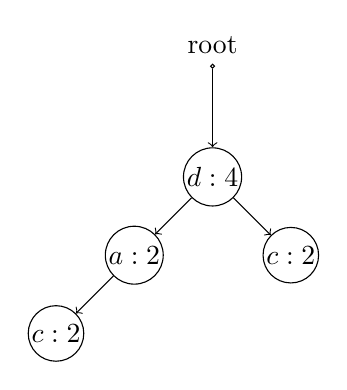
\begin{tikzpicture}[
			node distance=40pt,
			main/.style = {draw, circle, inner sep=.5pt}
		]
		\node[main, label=above:{root}] (r) {};
		% Level 1.
		\node[main, below of=r] (d) {$d:4$};
		% Level 2.
		\node[main, below right of=d] (dc) {$c:2$};
		\node[main, below left of=d] (da) {$a:2$};
		% Level 3.
		\node[main, below left of=da] (dac) {$c:2$};

		\draw[->] (r) to (d);
		\draw[->] (d) to (dc);
		\draw[->] (d) to (da);
		\draw[->] (da) to (dac);
	\end{tikzpicture}
\end{center}
Βλέπουμε ότι η συχνότητα του $a$ είναι $2$ οπότε το $\{a,c,d\}$ δεν είναι συχνό.
\\[8pt]
Συνεχίζουμε ομοίως με το στοιχείο $a$.
\begin{center}
	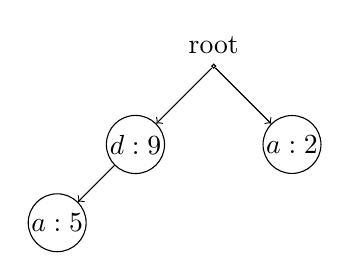
\begin{tikzpicture}[
			node distance=40pt,
			main/.style = {draw, circle, inner sep=.5pt}
		]
		\node[main, label=above:{root}] (r) {};
		% Level 1.
		\node[main, below left of=r] (d) {$d:9$};
		\node[main, below right of=r] (a) {$a:2$};
		% Level 2.
		\node[main, below left of=d] (da) {$a:5$};
		
		\draw[->] (r) to (d);
		\draw[->] (r) to (a);
		\draw[->] (d) to (da);
	\end{tikzpicture}
	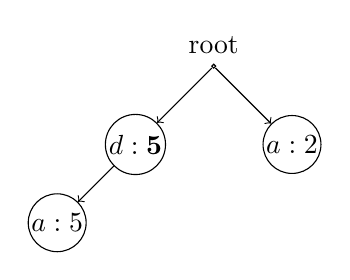
\begin{tikzpicture}[
			node distance=40pt,
			main/.style = {draw, circle, inner sep=.5pt}
		]
		\node[main, label=above:{root}] (r) {};
		% Level 1.
		\node[main, below left of=r] (d) {$d:\mathbf{5}$};
		\node[main, below right of=r] (a) {$a:2$};
		% Level 2.
		\node[main, below left of=d] (da) {$a:5$};
		
		\draw[->] (r) to (d);
		\draw[->] (r) to (a);
		\draw[->] (d) to (da);
	\end{tikzpicture}
\end{center}
Εφόσον η συχνότητα του $d$ είναι $5$ παίρνουμε ότι το $\{a,d\}$ συχνό.
Εφόοσον το υποδέντρο έχει μόνο δύο στοιχεία δεν έχει νόημα να ψάξουμε για 3-itemsets, ενώ για τον ίδιο λόγο δεν έχει νόημα να κοιτάξουμε το στοιχείο $d$ (το υποδέντρο θα έχει μόνο έναν κόμβο πέρα από το root).
\\[8pt]
Οπότε τα συχνά υποσύνολα της βάσης δεδομένων είναι τα
\[ \{ \{a,c\},\{a,d\},\{b,d\},\{c,d\} \} \]

\paragraph{(ε)}
\subparagraph{$s^\prime=1$} Με threshold $s^\prime$ από τις 3 πρώτες εγγραφές παίρνουμε ότι τα υποψήφια συχνά itemets είναι τα
\[ \{a,c,d\},\{b,c,d\} \]
προφανώς μαζί με όλα τα υποσύνολά τους.
Το Negative Border είναι το σύνολο $\{ \{a,b\} \}$ εφόσον αυτό είναι το μοναδικό 2-itemset που δεν είναι συχνό (τα 1-itemsets είναι όλα συχνά), ενώ τα 3-itemsets που δεν είναι συχνά είναι τα $\{a,b,c\},\{a,b,d\}$ τα οποία και τα δύο έχουν υποσύνολο το $\{a,b\}$.
Τέλος προφανώς και το 4-itemset $\{a,b,c,d\}$ επίσης δεν είναι στο Negative Border.

Με έναν έλεγχο στη βάση βλέπουμε ότι ο αλγόριθμος θα βρει σωστά τα συχνά itemsets αφού όλα βρίσκονται στα υποψήφια ενώ το Negative Border θα βγει μη συχνό.

\subparagraph{$s^{\prime\prime}=2$} Με threshold $s^{\prime\prime}$ από τις 3 πρώτες εγγραφές παίρνουμε ότι τα υποψήφια συχνά itemsets είναι τα
\[ \{ \{c\},\{a,d\} \} \]
και το Negative Border είναι το
\[ \{ \{b\},\{a,c\},\{c,d\} \} \]
Βλέπουμε ότι ο αλγόριθμος δεν θα δουλέψει διότι το $\{b\}$ από το Negative Border είναι συχνό itemset στη βάση.
\\[8pt]
Παρατηρούμε ότι όπως περιμέναμε το $s^{\prime\prime}$ δεν ήταν καλή επιλογή για threshold.
Εφόσον πήραμε το $1/4$ των εγγραφών για δείγμα, το προτεινόμενο θα ήταν να πάρουμε ένα ακόμα μικρότερο κλάσμα του αρχικού threshold.
Αυτό εδώ προφανώς δεν γίνεται οπότε το $s^\prime$, το ακριβώς $1/4$ του $s$, είναι μια καλή επιλογή που εσωκλείει όλα τα συχνά στα υποψήφια, ενώ το $s^{\prime\prime}$ αφήνει τα περισσότερα απ' έξω.

\section*{Άσκηση 5}

\subsection*{7.2.2 (MMDS)}

\paragraph{(a)} Θα χρησιμοποιήσουμε το κριτήριο της ελάχιστης απόστασης δύο οποιοδήποτε σημείων μεταξύ δύο clusters στο παράδειγμα 7.2 του MMDS.
Για το συγκεκριμένο κριτήριο συμφέρει να υπολογίσουμε έναν πίνακα που να περιέχει όλες τις αποστάσεις μεταξύ των σημείων, και από εκεί να ψάξουμε την μικρότερη τιμή όπου τα σημεία δεν ανήκουν στον ίδιο cluster για να κάνουμε τα merges.
Σε αντίθεση με το κριτήριο κοντινότερου centroid, ένα merge δεν αλλάζει τις αποστάσεις που θα πρέπει να συγκρίνουμε.
Οπότε τα merges γίνονται ως εξής
\begin{center}
	\begin{tabular}{| c | c || c | c |}
		\hline
		points & distance & points & distance \\ \hhline{|=|=#=|=|}
		$(10,5),(11,4)$ & $\sqrt{2}$ & $(6,8),(7,10)$ & $\sqrt{5}$ \\ \hline
		$(11,4),(12,3)$ & $\sqrt{2}$ & $(10,5),(12,6)$ & $\sqrt{5}$ \\ \hline
		$(4,8),(4,10)$ & $2$ & $(9,3),(10,5)$ & $\sqrt{5}$\\ \hline
		$(4,8),(6,8)$ & $2$ & $(2,2),(3,4)$ & $\sqrt{5}$ \\ \hline
		& & $(5,2),(3,4)$ & $\sqrt{5}$ \\ \hline
	\end{tabular}
\end{center}
με τα οποία οι τελικοί clusters είναι οι ίδιοι με το παράδειγμα, δηλαδή τρεις clusters
\[ \{ (4,10),(7,10),(4,8),(6,8) \}, \{ (10,5),(12,6),(11,4),(9,3),(12,3) \}, \{ (3,4),(2,2),(5,2) \} \]

\paragraph{(b)}
Θα χρησιμοποιήσουμε το κριτήριο της μέσης απόστασης δύο σημείων μεταξύ δύο clusters στο παράδειγμα 7.2 του MMDS.
Θα χρησιμοποιήσουμε πάλι τον πίνακα με όλες τις αποστάσεις των σημείων για να υπολογίσουμε τη μέση απόσταση μεταξύ δύο clusters.
Επίσης μπορούμε να παρατηρήσουμε ότι η μέση απόσταση είναι μεγαλύτερη ή ίση από την ελάχιστη απόσταση μεταξύ δυο σημείων, ένα από κάθε cluster (κριτήριο στο (a)), οπότε μπορούμε να αποφύγουμε κάποιους υπολογισμούς.
Τα merges λοιπόν γίνονται ως εξής
\begin{center}
	\begin{tabular}{| c | c |}
		\hline
		clusters & av. distance \\ \hhline{|=|=|}
		$\{(10,5)\},\{(11,4)\}$ & $\sqrt{2}$ \\ \hline
		$\{(4,8)\},\{(4,10)\}$ & $2$ \\ \hline
		$\{(10,5),(11,4)\},\{(12,3)\}$ & $(\sqrt{2}+\sqrt{8})/2$ \\ \hline
		$\{(6,8)\},\{(7,10)\}$ & $\sqrt{5}$ \\ \hline
		$\{(2,2)\},\{(3,4)\}$ & $\sqrt{5}$ \\ \hline
		$\{(10,5),(11,4)\},(12,3)\},\{(9,3)\}$ & $(\sqrt{5}+\sqrt{5}+3)/3$ \\ \hline
		$\{(2,2),(3,4)\},\{(5,2)\}$ & $(\sqrt{5}+3)/2$ \\ \hline
		$\{(4,8),(4,10)\},\{(6,8),(7,10)\}$ & $(2+\sqrt{8}+3+\sqrt{13})/4$ \\ \hline
		$\{(10,5),(11,4)\},(12,3),(9,3)\},\{(12,6)\}$ & $(\sqrt{5}+\sqrt{5}+3+\sqrt{18})/4$ \\ \hline
	\end{tabular}
\end{center}
με τα οποία οι τελικοί clusters είναι πάλι οι ίδιοι με προηγουμένως
\[ \{ (4,10),(7,10),(4,8),(6,8) \}, \{ (10,5),(12,6),(11,4),(9,3),(12,3) \}, \{ (3,4),(2,2),(5,2) \} \]

\subsection*{7.2.3 (MMDS)}

\paragraph{(a)} Θα χρησιμοποιήσουμε το κριτήριο της ελάχιστης ακτίνας στο παράδειγμα 7.2 του MMDS.
Θεωρούμε ως ακτίνα ενός cluster τη μέγιστη απόσταση ενός σημείου του με το centroid.
Λόγω απαιτητικών υπολογισμών η παρακάτω ακολουθία cluster merges υπολογίστηκε μέσω Python script.

\begin{center}
	\begin{tabular}{| c | c | c |}
		\hline
		clusters & centroid & radius \\ \hhline{|=|=|=|}
		$\{(10,5)\},\{(11,4)\}$ & $(10.5,4.5)$ & $0.7$ \\ \hline
		$\{(4, 10)\},\{(4, 8)\}$ & $(4.0, 9.0)$ & $1.0$ \\ \hline
		$\{(7, 10)\},\{(6, 8)\}$ & $(6.5, 9.0)$ & $1.12$ \\ \hline
		$\{(3, 4)\},\{(2, 2)\}$ & $(2.5, 3.0)$ & $1.12$ \\ \hline
		$\{(12, 6)\},\{(10, 5), (11, 4)\}$ & $(11.0, 5.0)$ & $1.41$ \\ \hline
		$\{(9, 3)\},\{(12, 3)\}$ & $(10.5, 3.0)$ & $1.5$ \\ \hline
		$\{(5, 2)\},\{(3, 4), (2, 2)\}$ & $(3.33, 2.67)$ & $1.8$ \\ \hline
		$\{(4, 10), (4, 8)\},\{(7, 10), (6, 8)\}$ & $(5.25, 9.0)$ & $2.02$ \\ \hline
		$\{(12, 6), (10, 5), (11, 4)\},\{(12, 3), (9, 3)\}$ & $(10.8, 4.2)$ & $2.16$ \\ \hline
	\end{tabular}
\end{center}
όπου καταλήγουμε πάλι στους γνωστούς τρεις clusters
\[ \{ (4,10),(7,10),(4,8),(6,8) \}, \{ (10,5),(12,6),(11,4),(9,3),(12,3) \}, \{ (3,4),(2,2),(5,2) \} \]



\paragraph{(b)} Θα χρησιμοποιήσουμε το κριτήριο της ελάχιστης διαμέτρου στο παράδειγμα 7.2 του MMDS.
Θεωρούμε ως διάμετρο ενός cluster τη μέγιστη απόσταση μεταξύ δύο οποιονδήποτε σημείων του.
Mέσω Python script παίρνουμε τα παρακάτω cluster merges.
\begin{center}
	\begin{tabular}{| c | c |}
		\hline
		clusters & diameter \\ \hhline{|=|=|}
		$\{(10, 5)\},\{(11, 4)\}$ & $1.41$ \\ \hline
		$\{(4, 10)\},\{(4, 8)\}$ & $2.0$ \\ \hline
		$\{(7, 10)\},\{(6, 8)\}$ & $2.24$ \\ \hline
		$\{(12, 6)\},\{(10, 5), (11, 4)\}$ & $2.24$ \\ \hline
		$\{(3, 4)\},\{(2, 2)\}$ & $2.24$ \\ \hline
		$\{(9, 3)\},\{(12, 3)\}$ & $3.0$ \\ \hline
		$\{(5, 2)\},\{(3, 4), (2, 2)\}$ & $3.0$ \\ \hline
		$\{(4, 10), (4, 8)\},\{(7, 10), (6, 8)\}$ & $3.61$ \\ \hline
		$\{(12, 6), (10, 5), (11, 4)\},\{(12, 3), (9, 3)\}$ & $4.24$ \\ \hline
	\end{tabular}
\end{center}
όπου καταλήγουμε πάλι στους γνωστούς τρεις clusters
\[ \{ (4,10),(7,10),(4,8),(6,8) \}, \{ (10,5),(12,6),(11,4),(9,3),(12,3) \}, \{ (3,4),(2,2),(5,2) \} \]

%\subsection*{7.3.2 (MMDS)}

%Έστω $A,B,C$ οι τρεις clusters του παραδείγματος, δηλαδή
%\begin{flalign*}
%	A &= \{ (4,10),(7,10),(4,8),(6,8) \} \\
%	B &= \{ (10,5),(12,6),(11,4),(9,3),(12,3) \} \\
%	C &= \{ (3,4),(2,2),(5,2) \}
%\end{flalign*}
%Μετά όπως βλέπουμε από τον πίνακα της 7.2.2 (b) (τρεις τελευταίες γραμμές), οι διάμετροι των $A,B,C$ %είναι $3.61,4.24,3$ αντίστοιχα.
%Τώρα για το minimum intercluster distance βρίσκουμε
%\[ A,B:5 \qquad A,C:4.12 \qquad B,C:4.12 \]

\subsection*{7.4.1 (MMDS)}

Έστω $K$ το κοινό centroid των δύο clusters που έχουμε (κύκλο και δακτύλιο).
Εφόσον τα representative points είναι στα όριά τους, τότε ένα τέτοιο point από τον κύκλο θα έχει απόσταση $c$ από το $K$ ενώ αν είναι από το δακτύλιο τότε θα έχει είτε $i$ είτε $o$ ανάλογα αν είναι στο inner ή outer boundary.
Άρα το κοντινότερο που θα μπορούσαν να είναι δύο σημεία, ένα από κάθε cluster, είναι εάν βρίσκονται στην ίδια ευθεία με το $K$, στο ίδιο ημικύκλιο και το σημείο του δακτυλίου να είναι στο inner boundary, και άρα θα έχουν απόσταση $i-c$.

Προχωρώντας στο βήμα της μετακίνησης των σημείων στο $20\%$ της απόστασή τους από το centroid, η παραπάνω απόσταση προσαρμόζεται αντίστοιχα ως εξής
\[ \frac{20}{100}i-\frac{20}{100}c = \frac{1}{5}(i-c) \]
Οπότε εάν ισχύει ότι $1/5(i-c)<d$, ή αλλιώς
\[ i-c < 5d \]
τότε είναι πιθανό να υπάρχουν σημεία που θα ικανοποιούν τις παραπάνω συνθήκες και θα κάνουν trigger την συνθήκη που κάνει merge τους δύο clusters.
\\[8pt]
Στη συνέχεια μπορούμε να κάνουμε τη συνθήκη πιο αυστηρή εξετάζοντας τη μεγαλύτερη πιθανή απόσταση δύο σημείων, ένα από κάθε cluster, το οποίο συμβαίνει όταν πάλι τα σημεία είναι στην ίδια ευθεία με το $K$ αλλά σε αντίθετα ημισφαίρια (οπότε θα προσθέσουμε τις ακτίνες τους) και το σημείο του δακτυλίου να βρίσκεται στο outer boundary (ακτίνα $o$).
Τότε με την ίδια λογική όπως και παραπάνω παίρνουμε ότι οι δύο clusters θα γίνουν σίγουρα merge όταν
\[ o+c < 5d \]

\end{document}
